\documentclass[11pt]{article}
\usepackage[a4paper,margin=1in]{geometry}
\usepackage[T1]{fontenc}
\usepackage{lmodern}
\usepackage{microtype}
\usepackage{amsmath,amssymb,amsthm,mathtools,bm}
\usepackage{booktabs,array,tabularx,longtable}
\usepackage{enumitem}
\usepackage{xcolor}
\usepackage{tikz}
\usetikzlibrary{arrows.meta,positioning,shapes.geometric,fit,calc}
\usepackage[most]{tcolorbox}
\usepackage[hidelinks]{hyperref}
\usepackage[nameinlink,noabbrev]{cleveref}

\definecolor{navy}{HTML}{17365D}
\definecolor{blue}{HTML}{DCEAF7}
\definecolor{green}{HTML}{E2F0D9}
\definecolor{orange}{HTML}{FCE4D6}
\definecolor{graybox}{HTML}{F3F5F7}
\hypersetup{colorlinks=true,linkcolor=navy,citecolor=navy,urlcolor=navy}
\setlist{nosep,leftmargin=*}
\setlength{\parindent}{1.25em}
\setlength{\parskip}{0.25em}

\newcommand{\E}{\mathcal E}
\newcommand{\R}{\mathcal R}
\newcommand{\D}{\mathrm D}
\newcommand{\pr}{\operatorname{pr}}
\newcommand{\eps}{\varepsilon}
\newcommand{\dd}{\,\mathrm d}
\newcommand{\norm}[1]{\left\lVert#1\right\rVert}

\newtheorem{definition}{Definition}[section]
\newtheorem{proposition}[definition]{Proposition}
\newtheorem{theorem}[definition]{Theorem}
\newtheorem{lemma}[definition]{Lemma}
\newtheorem{assumption}[definition]{Assumption}
\newtheorem{remark}[definition]{Remark}

\newtcolorbox{instruction}[1]{
  colback=blue,colframe=navy,fonttitle=\bfseries,title={#1},
  boxrule=0.6pt,arc=1.5mm,left=1.5mm,right=1.5mm,top=1mm,bottom=1mm}
\newtcolorbox{warningbox}[1]{
  colback=orange,colframe=orange!45!black,fonttitle=\bfseries,title={#1},
  boxrule=0.6pt,arc=1.5mm,left=1.5mm,right=1.5mm,top=1mm,bottom=1mm}

\title{Approximate Lie-Symmetry Reduction and Certified Neural Correction\\
for Parameter-Perturbed Nonlinear PDEs}
\author{Carl\\WKU MATH 4890}
\date{Research manuscript draft, 2027 project}

\begin{document}
\maketitle

\begin{abstract}
We develop a reproducible workflow for nonlinear partial differential equations whose Lie point-symmetry algebra changes at a distinguished parameter value.  The workflow computes the exact symmetry algebra, records the finite symmetry maps $S_i(\eps)=\exp(\eps X_i)$, classifies inequivalent one-dimensional reductions, and converts a selected invariant problem into an ordinary differential equation.  Near a symmetry-enhanced parameter, approximate Lie invariance produces a hierarchy of reduced correction equations.  A neural network is used only for the unresolved one-dimensional remainder, while initial data and known Taylor or perturbation terms are imposed analytically.  Under regular-branch and Lipschitz assumptions, a uniform reduced residual yields a profile-error estimate; the approximate-symmetry defect adds a separate, explicitly visible term to the lifted PDE residual.  The principal case is the Lagrangian Saint--Venant--Exner master equation with power-law sediment flux near $m=3$, where an additional scaling generator appears.  The paper is both a mathematical specification and an implementation guide: every numerical choice is treated as a convergence parameter rather than built into the method.
\end{abstract}

\noindent\textbf{Keywords.} Lie point symmetry; approximate symmetry; similarity reduction; Saint--Venant--Exner equation; physics-informed neural network; residual certificate.

\section{Problem and contribution}

Consider a parameter-dependent nonlinear PDE system
\begin{equation}
  \E_{\delta}[u]=0,
  \qquad (x,t)\in\Omega,
  \qquad \delta\in\mathcal P,
  \label{eq:general-pde}
\end{equation}
where $\delta$ may change both the admitted symmetries and the form of the reduced equations.  Directly fitting $u(x,t,\delta)$ treats every coordinate as an independent learning direction.  Our aim is to remove directions that are known analytically from the group action and learn only the remaining profile.

The central claim is conditional and testable.  Suppose exact or approximate symmetry coordinates reduce \cref{eq:general-pde} to an ODE for a profile $F$.  If a semi-analytic neural trial (i) satisfies the reduced data exactly, (ii) remains in a regular region, and (iii) has a uniformly bounded reduced residual, then its profile error can be bounded by ODE stability.  When the symmetry is approximate rather than exact, the lifted PDE residual contains a second term measuring symmetry breaking.  Thus optimization error and reduction error are reported separately.

This positioning is narrower than recent symmetry-informed neural solvers.  Continuous symmetries have been imposed through invariant architectures and transformed sampling \cite{zhang2023,akhound2024,arora2024}; symmetry reduction has also been coupled directly to PINNs for moving and rescaled frames \cite{kavousanakis2026}; Taylor polynomials with neural remainders have been developed for ODE families \cite{nagesh2025}.  Our focus is the junction of four steps: symmetry classification at a parameter singularity, approximate reduction after symmetry breaking, a one-dimensional neural correction, and a lifted error statement.

\begin{figure}[t]
\centering
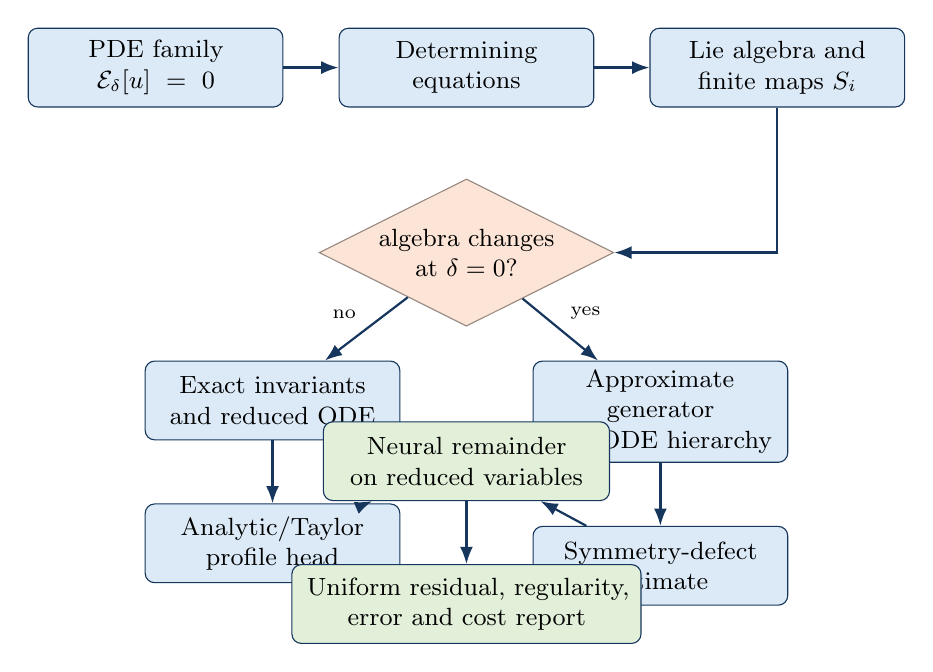
\begin{tikzpicture}[
  node distance=5mm and 7mm,
  box/.style={draw=navy,rounded corners=1.2mm,fill=blue,align=center,
              minimum height=10mm,text width=30mm,font=\small},
  test/.style={draw=orange!60!black,diamond,aspect=2.0,fill=orange,
               align=center,font=\small,inner sep=1.4pt},
  arr/.style={-{Latex[length=2.2mm]},thick,draw=navy}
]
\node[box] (model) {PDE family\\$\E_\delta[u]=0$};
\node[box,right=of model] (det) {Determining\\equations};
\node[box,right=of det] (alg) {Lie algebra and\\finite maps $S_i$};
\node[test,below=9mm of det] (enh) {algebra changes\\at $\delta=0$?};
\node[box,below left=9mm and -1mm of enh] (exact) {Exact invariants\\and reduced ODE};
\node[box,below right=9mm and -1mm of enh] (approx) {Approximate generator\\and ODE hierarchy};
\node[box,below=8mm of exact] (head) {Analytic/Taylor\\profile head};
\node[box,below=8mm of approx] (defect) {Symmetry-defect\\estimate};
\node[box,below=12mm of enh,text width=34mm,fill=green] (nn) {Neural remainder\\on reduced variables};
\node[box,below=8mm of nn,text width=42mm,fill=green] (cert) {Uniform residual, regularity,\\error and cost report};
\draw[arr] (model)--(det);
\draw[arr] (det)--(alg);
\draw[arr] (alg.south) |- (enh.east);
\draw[arr] (enh)--node[above left,font=\scriptsize]{no}(exact);
\draw[arr] (enh)--node[above right,font=\scriptsize]{yes}(approx);
\draw[arr] (exact)--(head);
\draw[arr] (approx)--(defect);
\draw[arr] (head)--(nn);
\draw[arr] (defect)--(nn);
\draw[arr] (nn)--(cert);
\end{tikzpicture}
\caption{The proposed workflow.  The network enters after symmetry analysis and dimensional reduction.}
\label{fig:pipeline}
\end{figure}

\section{Lie point symmetries: the complete reduction workflow}

\subsection{Point transformations, generators, and finite maps}

For two independent variables $(t,s)$ and one dependent variable $\phi$, a local one-parameter point transformation has the form
\begin{equation}
 (\bar t,\bar s,\bar\phi)
 =S_X(\eps)(t,s,\phi),
 \qquad S_X(0)=\operatorname{id}.
 \label{eq:finite-group}
\end{equation}
Its infinitesimal generator is
\begin{equation}
 X=\tau(t,s,\phi)\partial_t+\xi(t,s,\phi)\partial_s
   +\eta(t,s,\phi)\partial_\phi,
 \qquad
 S_X(\eps)=\exp(\eps X).
 \label{eq:generator}
\end{equation}
For a basis generator $X_i$, we write
\begin{equation}
 S_i(\eps):=S_{X_i}(\eps)=\exp(\eps X_i).
 \label{eq:Si}
\end{equation}
The notation matters: $X_i$ is a vector field, while $S_i(\eps)$ is the actual transformation acting on points and solutions.

Let $J=(j_1,\ldots,j_k)$ be a derivative multi-index and let
\begin{equation}
 Q=\eta-\tau\phi_t-\xi\phi_s
 \label{eq:characteristic}
\end{equation}
be the characteristic of $X$.  A convenient prolongation formula is
\begin{equation}
 \eta_J=\D_JQ+\tau\phi_{J,t}+\xi\phi_{J,s},
 \qquad
 \pr^{(n)}X=X+\sum_{1\le |J|\le n}\eta_J\partial_{\phi_J}.
 \label{eq:prolongation}
\end{equation}
If $H(t,s,\phi^{(n)};\delta)=0$ is an $n$th-order PDE, the infinitesimal invariance criterion is
\begin{equation}
 \left.\pr^{(n)}X(H)\right|_{H=0}=0.
 \label{eq:invariance}
\end{equation}

\begin{instruction}{Lie analysis in five operations}
Write the most general point generator.  Prolong it to the highest derivative in the PDE.  Apply \cref{eq:invariance}.  Eliminate one leading derivative using the PDE, split the resulting identity with respect to the remaining independent jet variables, and solve the resulting linear determining equations for $(\tau,\xi,\eta)$.
\end{instruction}

\subsection{Algebra, adjoint equivalence, and an optimal system}

The admitted generators form a Lie algebra under
\begin{equation}
 [X,Y]=XY-YX.
\end{equation}
Two one-dimensional subalgebras generate equivalent reductions if they are related by scaling and the adjoint action.  The calculation uses
\begin{equation}
 \operatorname{Ad}(\exp(\eps X_i))X_j
 =X_j-\eps[X_i,X_j]+\frac{\eps^2}{2}[X_i,[X_i,X_j]]+\cdots.
 \label{eq:adjoint}
\end{equation}
An optimal system is a list of representatives, one from each relevant adjoint orbit.  This step prevents the same similarity reduction from being rediscovered in different coordinates.

For a representative
\begin{equation}
 X=\tau\partial_t+\xi\partial_s+\eta\partial_\phi,
\end{equation}
solve the characteristic equations
\begin{equation}
 \frac{\dd t}{\tau}=\frac{\dd s}{\xi}=\frac{\dd\phi}{\eta}.
 \label{eq:characteristic-system}
\end{equation}
Two independent first integrals give an invariant coordinate and an invariant dependent-variable combination.  Substitution converts a PDE in $(t,s)$ into an ODE in the invariant coordinate.

\begin{figure}[t]
\centering
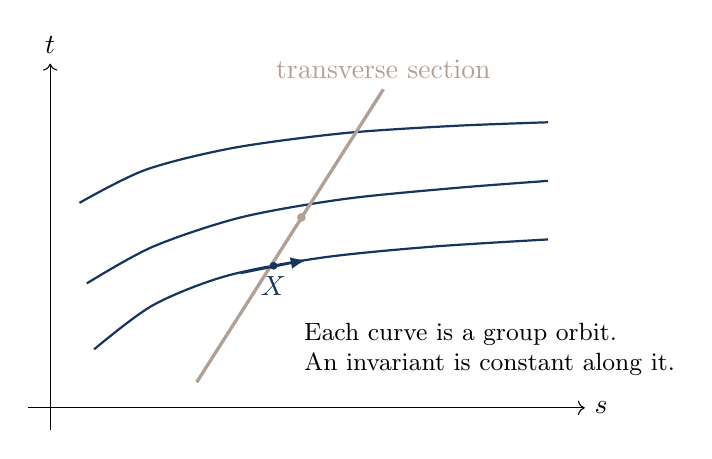
\begin{tikzpicture}[scale=0.93,
  orbit/.style={navy,thick},
  arr/.style={-{Latex[length=2mm]},navy,thick}]
  \draw[->] (-0.3,0)--(7.3,0) node[right]{$s$};
  \draw[->] (0,-0.3)--(0,4.7) node[above]{$t$};
  \draw[orbit] plot[smooth] coordinates{(0.6,0.8)(1.4,1.4)(2.4,1.8)(3.7,2.05)(5.2,2.2)(6.8,2.3)};
  \draw[orbit] plot[smooth] coordinates{(0.5,1.7)(1.4,2.2)(2.6,2.6)(4.0,2.85)(5.5,3.0)(6.8,3.1)};
  \draw[orbit] plot[smooth] coordinates{(0.4,2.8)(1.3,3.25)(2.5,3.55)(4.0,3.75)(5.5,3.85)(6.8,3.9)};
  \draw[orange!70!black,very thick] (2.0,0.35)--(4.55,4.35) node[above]{transverse section};
  \draw[arr] (2.6,1.84)--(3.5,2.02) node[midway,below]{$X$};
  \fill[navy] (3.05,1.94) circle(1.5pt);
  \fill[orange!70!black] (3.43,2.60) circle(1.7pt);
  \node[align=left,font=\small] at (6.0,0.8) {Each curve is a group orbit.\\An invariant is constant along it.};
\end{tikzpicture}
\caption{Geometric meaning of reduction.  A group orbit removes one independent direction; an invariant coordinate labels the orbits.}
\label{fig:orbits}
\end{figure}

\section{The Lagrangian Saint--Venant--Exner master equation}

\subsection{Model scope}

Following Paliathanasis, Leon, and Leach \cite{paliathanasis2026}, introduce the particle-position potential $\phi(t,s)$ through
\begin{equation}
 u=\phi_t,
 \qquad h=\frac{1}{\phi_s},
 \qquad u>0,\quad \phi_s>0.
\end{equation}
For the power-law sediment flux $Q=A_g u^m$, define $\beta=mA_g\zeta$, where $\zeta$ is the porosity factor used in the source.  The printed Lagrangian pair is
\begin{align}
 \phi_{tt}-g\frac{\phi_{ss}}{\phi_s^3}+\frac{g}{\phi_s}B_s&=0,\label{eq:pair1}\\
 B_t+\beta\phi_t^{m-1}\frac{\phi_{ts}}{\phi_s}&=0.\label{eq:pair2}
\end{align}
Differentiating and imposing equality of $B_{st}$ and $B_{ts}$ gives the master equation
\begin{equation}
 \E_m[\phi]
 :=\partial_t\!\left(\phi_s\phi_{tt}-g\frac{\phi_{ss}}{\phi_s^2}\right)
 -g\beta\partial_s\!\left(\phi_t^{m-1}\frac{\phi_{ts}}{\phi_s}\right)=0.
 \label{eq:master}
\end{equation}
Our mathematical target is \cref{eq:master}.  Reconstruction of $B$ from \cref{eq:pair1,eq:pair2} is valid locally on a simply connected regular region.  Any claim that the printed pair is equivalent to a separately formulated Eulerian bed equation requires an additional coordinate audit and is outside the theorem below.

\subsection{Exact admitted symmetries and the maps \texorpdfstring{$S_i(\eps)$}{Si(epsilon)}}

Solving the determining equations from \cref{eq:invariance} gives, for arbitrary $m$, the generators
\begin{equation}
 X_1=\partial_t,
 \qquad X_2=\partial_s,
 \qquad X_3=\partial_\phi,
 \qquad X_4=t\partial_t+s\partial_s+\phi\partial_\phi.
 \label{eq:generic-generators}
\end{equation}
Equivalently, the general solution of the split determining system is
\begin{equation}
 \tau=c_1+c_4t,\qquad
 \xi=c_2+c_4s,\qquad
 \eta=c_3+c_4\phi
 \qquad (m\ne3).
 \label{eq:generic-determining-solution}
\end{equation}
At $m=3$, the algebra enlarges by
\begin{equation}
 X_5=t\partial_t-2s\partial_s.
 \label{eq:X5}
\end{equation}
and the determining-system solution becomes
\begin{equation}
 \tau=c_1+(c_4+c_5)t,\qquad
 \xi=c_2+(c_4-2c_5)s,\qquad
 \eta=c_3+c_4\phi.
 \label{eq:special-determining-solution}
\end{equation}
The corresponding finite symmetry transformations are obtained by integrating
$\frac{\dd}{\dd\eps}S_i(\eps)z=X_i(S_i(\eps)z)$:
\begin{table}[ht]
\centering
\caption{Generators and finite symmetry maps.  These are the $S_i(X)$ requested in the project, written precisely as $S_i(\eps)=\exp(\eps X_i)$.}
\label{tab:finite-maps}
\begin{tabularx}{\textwidth}{@{}c l X c@{}}
\toprule
$i$ & generator $X_i$ & $S_i(\eps):(t,s,\phi)\mapsto(\bar t,\bar s,\bar\phi)$ & validity\\
\midrule
1 & $\partial_t$ & $(t+\eps,s,\phi)$ & all $m$\\
2 & $\partial_s$ & $(t,s+\eps,\phi)$ & all $m$\\
3 & $\partial_\phi$ & $(t,s,\phi+\eps)$ & all $m$\\
4 & $t\partial_t+s\partial_s+\phi\partial_\phi$
  & $(e^\eps t,e^\eps s,e^\eps\phi)$ & all $m$\\
5 & $t\partial_t-2s\partial_s$
  & $(e^\eps t,e^{-2\eps}s,\phi)$ & $m=3$\\
\bottomrule
\end{tabularx}
\end{table}

For example, $S_5(\eps)$ leaves $st^2$ unchanged:
\begin{equation}
 (e^{-2\eps}s)(e^\eps t)^2=st^2.
\end{equation}
The induced action on a graph is obtained with inverse coordinates:
\begin{equation}
 (S_5(\eps)\cdot\phi)(t,s)
 =\phi(e^{-\eps}t,e^{2\eps}s).
 \label{eq:solution-action}
\end{equation}
An invariant graph satisfies $S_5(\eps)\cdot\phi=\phi$, or infinitesimally
$t\phi_t-2s\phi_s=0$.  Solving this first-order equation gives
$\phi=F(st^2)$.
It is therefore the symmetry responsible for the main reduction.  The nonzero brackets in the basis convention of \cref{eq:generic-generators,eq:X5} are
\begin{equation}
\begin{aligned}
 [X_1,X_4]&=X_1, & [X_2,X_4]&=X_2, & [X_3,X_4]&=X_3,\\
 [X_1,X_5]&=X_1, & [X_2,X_5]&=-2X_2.
\end{aligned}
 \label{eq:brackets}
\end{equation}
These brackets, together with \cref{eq:adjoint}, determine inequivalent one-dimensional subalgebras.  A representative list includes
\begin{equation}
 \{X_1+\alpha_2X_2+\alpha_3X_3\},\quad
 \{X_4\},\quad \{X_5\},\quad \{X_4+\alpha X_5\},
 \label{eq:optimal}
\end{equation}
with parameter restrictions and degeneracies handled through the adjoint table \cite{paliathanasis2026}.  The project records the full table but develops $\{X_5\}$ because it is the symmetry-enhanced branch that disappears away from $m=3$.

\begin{instruction}{What must appear in a reproducible symmetry paper}
Report the determining equations or enough information to regenerate them; list the basis $X_i$; state every nonzero commutator; give the finite maps $S_i(\eps)$; explain adjoint equivalence; list the optimal representatives; and show the characteristic equations for every reduction used later.  A similarity ansatz without these steps is evidence of a reduction, not a complete Lie analysis.
\end{instruction}

\section{Exact reduction at the symmetry-enhanced exponent}

For $X_5$, \cref{eq:characteristic-system} becomes
\begin{equation}
 \frac{\dd t}{t}=\frac{\dd s}{-2s}=\frac{\dd\phi}{0}.
\end{equation}
Hence
\begin{equation}
 \sigma=st^2,
 \qquad \phi(t,s)=F(\sigma).
 \label{eq:invariant-ansatz}
\end{equation}
The derivatives needed for substitution are
\begin{align}
 \phi_s&=t^2F', & \phi_t&=2stF'=\frac{2\sigma}{t}F',\\
 \phi_{ss}&=t^4F'', & \phi_{ts}&=2t(F'+\sigma F''),\\
 \phi_{tt}&=2sF'+4s\sigma F''.
 \label{eq:derivatives}
\end{align}
Primes now denote $\dd/\dd\sigma$.  Direct substitution into \cref{eq:master} with $m=3$ gives
\begin{equation}
 \E_3[F(st^2)]=t^{-1}\R_3[F],
 \qquad
 \R_3[F]=a(\sigma,F')F'''+b(\sigma,F',F''),
 \label{eq:lift-exact}
\end{equation}
where
\begin{align}
 a(\sigma,r)&=8(1-g\beta)\sigma^3r-\frac{2g\sigma}{r^2},\label{eq:a}\\
 b(\sigma,r,v)&=4\sigma(1-4g\beta)r^2
 +8\sigma^2(3-5g\beta)rv\notag\\
 &\quad+\left[8\sigma^3(1-g\beta)+\frac{4g\sigma}{r^3}\right]v^2.
 \label{eq:b}
\end{align}
Thus the invariant PDE problem becomes the third-order ODE $\R_3[F]=0$.

On a regular branch
\begin{equation}
 r=F'>0,
 \qquad |a(\sigma,r)|\ge a_{\min}>0,
 \label{eq:regular-branch}
\end{equation}
the equation is equivalent to the first-order system
\begin{equation}
 Y'=G(\sigma,Y)
 :=\left(r,v,-\frac{b(\sigma,r,v)}{a(\sigma,r)}\right),
 \qquad Y=(F,r,v).
 \label{eq:first-order}
\end{equation}
The conditions in \cref{eq:regular-branch} are mathematical assumptions to verify, not penalties that may silently fail.

An exact control profile is
\begin{equation}
 F_0(\sigma)=K\sigma^{1/3},
 \qquad K^3=\frac{27g}{1-4g\beta},
 \label{eq:control}
\end{equation}
whenever the parameters and branch make $K$ real and the regularity conditions hold.  This profile is used to check symbolic differentiation, numerical convergence, and lifting.

\section{Symmetry breaking near \texorpdfstring{$m=3$}{m=3}}

Let
\begin{equation}
 m=3+\delta,
 \qquad |\delta|\ll1.
 \label{eq:delta}
\end{equation}
The added generator $X_5$ is no longer exact when $\delta\ne0$.  This is the source of the research problem rather than a nuisance to hide.

Define
\begin{equation}
 A=\phi_s\phi_{tt}-g\frac{\phi_{ss}}{\phi_s^2},
 \qquad
 q_m=\phi_t^{m-1}\frac{\phi_{ts}}{\phi_s},
 \qquad \E_m=A_t-g\beta(q_m)_s.
\end{equation}
Under $S_5(\eps)$, $A_t$ has scaling weight $-1$, while $(q_m)_s$ has weight $2-m$.  Therefore:

\begin{proposition}[Exact symmetry-defect identity]
On the solution manifold $\E_m=0$,
\begin{equation}
 \left.\pr^{(3)}X_5(\E_m)\right|_{\E_m=0}
 =g\beta(m-3)(q_m)_s.
 \label{eq:defect-identity}
\end{equation}
Consequently, $X_5$ is exact at $m=3$ and is a zeroth-order approximate symmetry with an $O(\delta)$ defect on compact regular sets when $m=3+\delta$.
\end{proposition}

\begin{proof}
The derivative weights are $w(\partial_t)=-1$, $w(\partial_s)=2$, and $w(\phi)=0$.  Hence $w(A_t)=-1$ and $w((q_m)_s)=2-m$.  It follows that
\[
 \pr^{(3)}X_5(\E_m)=-A_t-g\beta(2-m)(q_m)_s.
\]
Using $A_t=g\beta(q_m)_s$ on $\E_m=0$ gives \cref{eq:defect-identity}.
\end{proof}

When $\phi_t>0$,
\begin{equation}
 \phi_t^{2+\delta}
 =\phi_t^2\exp(\delta\log\phi_t)
 =\phi_t^2\sum_{k=0}^{p}\frac{\delta^k}{k!}(\log\phi_t)^k
 +O(\delta^{p+1}).
 \label{eq:power-expansion}
\end{equation}
For the exact invariant coordinate $\sigma=st^2$, $\phi_t=2\sigma F'/t$; therefore $\log\phi_t$ contains $-\log t$.  This explains why substituting $F(st^2)$ at $m\ne3$ does not produce a pure ODE.  A consistent approximate reduction must allow logarithmic correction modes.

We use the finite hierarchy
\begin{equation}
 \phi^{[p]}(t,s;\delta)
 =\sum_{k=0}^{p}\delta^k
   \sum_{\ell=0}^{k}(\log t)^\ell F_{k\ell}(\sigma),
 \qquad \sigma=st^2,
 \label{eq:hierarchy-ansatz}
\end{equation}
on domains with $0<t_-\le t\le t_+$.  Substitute \cref{eq:hierarchy-ansatz} into \cref{eq:master}, use \cref{eq:power-expansion}, and collect each coefficient of $\delta^k(\log t)^\ell$.  At $k=0$ one obtains \cref{eq:lift-exact}.  At higher orders one obtains linearized ODEs for $F_{k\ell}$ with forcing determined by lower orders.  The compatibility of this hierarchy is the first analytical task of the project.

A more general approximate generator
\begin{equation}
 X_\delta=X_5+\delta X^{(1)}+\cdots+\delta^pX^{(p)}
 \label{eq:approx-generator}
\end{equation}
may be sought using the approximate-group method of Baikov, Gazizov, and Ibragimov \cite{baikov1989}.  With
\begin{equation}
 \E_\delta=\E_0+\delta\E_1+\cdots,
\end{equation}
the order-$k$ determining equations come from
\begin{equation}
 \left.\sum_{j=0}^{k}\pr^{(3)}X^{(j)}(\E_{k-j})\right|_{\E_0=0}=0
 \quad\text{modulo lower-order equations}.
 \label{eq:approx-determining}
\end{equation}
If no nontrivial $X^{(1)}$ solves this system, the negative result is informative: the logarithmic hierarchy \cref{eq:hierarchy-ansatz}, rather than a deformed exact similarity variable, becomes the correct reduction object.

\begin{warningbox}{Do not call $F(st^2)$ an exact reduction for $m\ne3$}
The extra scaling symmetry exists only at $m=3$.  Away from that exponent, a pure similarity ansatz leaves explicit $t$-dependence.  The paper must report the resulting defect or construct an approximate generator; otherwise the reduced model solves a different equation.
\end{warningbox}

\section{Semi-analytic neural correction}

\subsection{What the network learns}

The network does not relearn the symmetry map, the invariant coordinate, known perturbation coefficients, or initial data.  After truncating the analytical hierarchy at order $p$, write schematically
\begin{equation}
 \widehat\phi_\theta
 =\phi^{[p]}+\delta^{p+1}\mathcal B(t,s,\delta)
   N_\theta(\sigma,\delta).
 \label{eq:neural-lift}
\end{equation}
The factor $\mathcal B$ enforces homogeneous correction data.  If the reduced profile is specified by
\begin{equation}
 F(\sigma_0)=F_*,\qquad F'(\sigma_0)=r_*,\qquad F''(\sigma_0)=v_*,
 \label{eq:profile-data}
\end{equation}
a scalar exact-data trial at $m=3$ is
\begin{equation}
 \widehat F_\theta(\sigma)
 =F_*+r_*z+\frac12v_*z^2+z^3N_\theta(\widehat\sigma),
 \qquad z=\sigma-\sigma_0,
 \label{eq:hard-trial}
\end{equation}
where $\widehat\sigma$ is a nondimensionalized coordinate, normally mapped to $[-1,1]$.  Higher Taylor coefficients may be computed recursively from \cref{eq:first-order} and inserted before the neural term.

\begin{figure}[t]
\centering
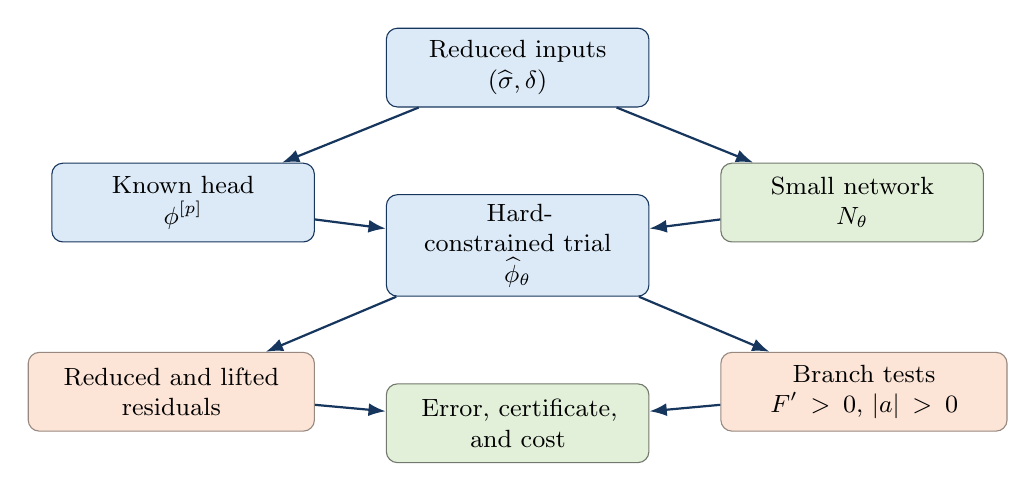
\begin{tikzpicture}[
 node distance=7mm and 9mm,
 b/.style={draw=navy,rounded corners,fill=blue,align=center,minimum height=10mm,text width=31mm,font=\small},
 g/.style={draw=green!50!black,rounded corners,fill=green,align=center,minimum height=10mm,text width=31mm,font=\small},
 o/.style={draw=orange!60!black,rounded corners,fill=orange,align=center,minimum height=10mm,text width=34mm,font=\small},
 a/.style={-{Latex[length=2.2mm]},thick,draw=navy}
]
\node[b] (coord) {Reduced inputs\\$(\widehat\sigma,\delta)$};
\node[b,below left=of coord] (analytic) {Known head\\$\phi^{[p]}$};
\node[g,below right=of coord] (net) {Small network\\$N_\theta$};
\node[b,below=11mm of coord] (trial) {Hard-constrained trial\\$\widehat\phi_\theta$};
\node[o,below left=of trial] (res) {Reduced and lifted\\residuals};
\node[o,below right=of trial] (reg) {Branch tests\\$F'>0$, $|a|>0$};
\node[g,below=11mm of trial] (report) {Error, certificate,\\and cost};
\draw[a] (coord)--(analytic);
\draw[a] (coord)--(net);
\draw[a] (analytic)--(trial);
\draw[a] (net)--(trial);
\draw[a] (trial)--(res);
\draw[a] (trial)--(reg);
\draw[a] (res)--(report);
\draw[a] (reg)--(report);
\end{tikzpicture}
\caption{The neural model learns a reduced correction.  Analytic constraints enter through the trial function, not through loosely weighted penalties.}
\label{fig:network}
\end{figure}

\subsection{Residuals and loss}

At $m=3$, compute both the raw residual
\begin{equation}
 R_{\rm raw}(\sigma;\theta)
 =a(\sigma,\widehat F_\theta')\widehat F_\theta'''
  +b(\sigma,\widehat F_\theta',\widehat F_\theta'')
 \label{eq:raw-residual}
\end{equation}
and the normalized residual
\begin{equation}
 R_{\rm ode}(\sigma;\theta)
 =\widehat F_\theta'''
  +\frac{b(\sigma,\widehat F_\theta',\widehat F_\theta'')}
        {a(\sigma,\widehat F_\theta')}.
 \label{eq:normalized-residual}
\end{equation}
The normalized residual drives the ODE error estimate, while the raw residual is the quantity appearing in the exact PDE lift \cref{eq:lift-exact}.  For the perturbed hierarchy, use the coefficients of $\delta^k(\log t)^\ell$ as reduced residuals and also evaluate the full master residual of \cref{eq:neural-lift} on an independent test set.

After nondimensionalization, a basic training loss is
\begin{equation}
 \mathcal L(\theta)
 =\operatorname{mean}_{\sigma\in\mathcal C_{\rm train}}
    |R_{\rm ode}(\sigma;\theta)|^2
  +\lambda_{\rm reg}\mathcal L_{\rm reg}.
 \label{eq:loss}
\end{equation}
Here $\mathcal L_{\rm reg}$ is a barrier or failure rule that prevents entry into $F'\le0$ or $|a|\le a_{\rm floor}$.  The branch conditions must subsequently be checked on a dense independent grid or by interval bounds.  A sampled penalty is not a proof of regularity.

\begin{instruction}{Simple implementation recipe}
Choose a compact parameter set and a regular profile interval from the mathematics.  Map inputs and outputs to order-one scales.  Build the exact-data trial function.  Differentiate it with automatic differentiation.  Train on the reduced residual.  Reject nonregular runs.  Evaluate on new points, compare with a converged ODE solver, and attempt uniform residual verification only after training.
\end{instruction}

\subsection{No unexplained hyperparameters}

Network width, depth, collocation count, optimizer steps, and parameter samples are experimental controls.  They are selected through a declared convergence study, not embedded in the problem statement.  Let
\begin{equation}
 (W,L,N_c,N_\delta)
\end{equation}
denote width, depth, collocation count, and parameter count.  Increase them until the validation residual and reference error stabilize within a declared tolerance.  Report all tested values and all random seeds.  The interval $I=[\sigma_0,\sigma_1]$, the perturbation range $\mathcal P$, and physical coefficients are justified by regularity, physical data, or the chosen benchmark question.

\section{Residual certificates and PDE lifting}

We first state the ODE part independently of neural networks.

\begin{theorem}[Reduced residual-to-profile estimate]
Let $I=[\sigma_0,\sigma_1]$, let $G:I\times\mathcal K\to\mathbb R^d$ be continuous and $L$-Lipschitz in $Y$ on a compact convex set $\mathcal K$, and let $Y$ solve
\begin{equation}
 Y'=G(\sigma,Y),\qquad Y(\sigma_0)=Y_0.
\end{equation}
Suppose a differentiable trial $\widehat Y:I\to\mathcal K$ has the same initial value and satisfies
\begin{equation}
 \norm{\widehat Y'-G(\sigma,\widehat Y)}_\infty\le\rho.
\end{equation}
If the resulting bound stays inside the verified margin of $\mathcal K$, then
\begin{equation}
 \norm{\widehat Y(\sigma)-Y(\sigma)}
 \le
 \begin{cases}
 \dfrac{\rho}{L}\bigl(e^{L(\sigma-\sigma_0)}-1\bigr),&L>0,\\[2mm]
 \rho(\sigma-\sigma_0),&L=0.
 \end{cases}
 \label{eq:gronwall}
\end{equation}
\end{theorem}

\begin{proof}
Let $e=\widehat Y-Y$ and $d=\widehat Y'-G(\sigma,\widehat Y)$.  Then
\[
 \norm{e(\sigma)}
 \le\int_{\sigma_0}^{\sigma}
 \bigl(L\norm{e(\zeta)}+\rho\bigr)\dd\zeta.
\]
Gronwall's inequality gives \cref{eq:gronwall}; a first-exit argument justifies use of the local Lipschitz constant on $\mathcal K$.
\end{proof}

For \cref{eq:first-order}, $d=3$ and the third component of the defect is \cref{eq:normalized-residual}.  A useful certificate therefore requires four computed objects: a regular compact tube $\mathcal K$, a lower bound for $|a|$, an upper bound for $\|D_YG\|$, and a uniform residual bound.  Sampling supplies diagnostics but not these uniform bounds.

\begin{theorem}[Approximate reduction and lifted residual]
Let $\phi^{[p]}$ be an order-$p$ approximate reduction on
\begin{equation}
 \Omega_I=\{(t,s):t_-\le t\le t_+,\ st^2\in I\},\qquad t_->0,
\end{equation}
and suppose all trial derivatives lie in a compact regular set.  Assume the chain-rule lift from the reduced residual vector $R_{\rm red}$ to the PDE residual has operator bound $C_{\rm lift}$, and the truncated approximate-symmetry hierarchy has defect at most $C_{\rm sym}|\delta|^{p+1}$.  Then
\begin{equation}
 \norm{\E_{3+\delta}[\widehat\phi_\theta]}_{L^\infty(\Omega_I)}
 \le C_{\rm lift}\norm{R_{\rm red}}_{L^\infty(I)}
      +C_{\rm sym}|\delta|^{p+1}.
 \label{eq:lift-bound}
\end{equation}
If the reduced system also satisfies the hypotheses of the preceding theorem, its profile error obeys \cref{eq:gronwall} with the reduced residual bound.
\end{theorem}

\begin{proof}
Substitution of the truncated analytic-neural ansatz splits the PDE residual into the image of the reduced residual and the discarded symmetry/perturbation terms.  Apply the triangle inequality and the two assumed operator bounds.  The profile estimate follows from the preceding theorem.
\end{proof}

\begin{remark}
The constants in \cref{eq:lift-bound} must be computed for the chosen domain and parameter set.  The theorem does not claim that a trained network automatically has a small uniform residual, nor that a small PDE residual alone controls the error of an ill-posed PDE problem.
\end{remark}

\section{Experimental design}

The study proceeds in increasing difficulty.  Each stage has a mathematical pass condition before the next begins.

\begin{enumerate}[label=\textbf{Stage \arabic*.}]
\item \textbf{Symbolic audit at $m=3$.} Reproduce $X_1,\ldots,X_5$, their brackets, $S_i(\eps)$, the $X_5$ invariants, \cref{eq:a,eq:b}, and the exact control \cref{eq:control}.  Compare symbolic and automatic derivatives.
\item \textbf{Exact reduced benchmark.} Compare Taylor-only, direct numerical integration, a plain reduced PINN, and the analytic-head neural remainder on the same admissible IVP family.  Train no full $(t,s)$ PINN yet.
\item \textbf{First-order symmetry breaking.} Set $m=3+\delta$, derive the $O(\delta)$ determining equations and logarithmic correction ODEs, and quantify the truncation defect against the full master equation.
\item \textbf{Parameterized neural correction.} Give $(\sigma,\delta)$ to one network, train over a compact perturbation range, and test at unseen parameter values.  Compare with solving each reduced IVP separately.
\item \textbf{Two-dimensional ablation.} Only after the reduced method works, train a direct PINN for $\phi(t,s)$ with comparable error targets.  Compare accuracy, training cost, derivative cost, and failure rate.  This tests the value of reduction rather than assuming it.
\end{enumerate}

The principal baselines are a high-accuracy adaptive ODE solver, the truncated analytic approximation without a network, a neural reduced solution without an analytic head, and a direct PDE PINN.  Report profile errors in $F,F',F''$, raw and normalized residuals, lifted PDE residuals, regularity margins, wall-clock cost, function/gradient evaluations, and every seed.  Classical solvers may be faster; this is a valid outcome.

\begin{table}[t]
\centering
\caption{Quantities that determine the experiment.}
\label{tab:choices}
\begin{tabularx}{\textwidth}{@{}l X X@{}}
\toprule
Choice & mathematical justification & selection/reporting rule\\
\midrule
$m=3+\delta$ & algebra enlarges at $m=3$ & declare compact $\delta$ range; test unseen values\\
$I=[\sigma_0,\sigma_1]$ & regularity of $F'$ and $a$ & grow interval until branch or accuracy fails\\
$(g,\beta)$ & physical/model regime and real control profile & nondimensionalize; perform parameter sensitivity\\
Taylor order $p$ & available symbolic derivatives and target remainder & compare adjacent orders at equal cost\\
network size & approximation capacity & width/depth convergence study\\
collocation set & quadrature of reduced residual & refinement and independent validation\\
optimizer budget & computational cost & report histories and stopping rule\\
\bottomrule
\end{tabularx}
\end{table}

\section{Algorithmic guide}

\begin{instruction}{Algorithm 1: symbolic reduction}
\begin{enumerate}[label=\arabic*.]
\item Specify $\E_m$, dependent variables, parameter domain, and regularity assumptions.
\item Construct a general point generator and its prolongation.
\item Split the invariance identity and solve the determining equations for generic $m$ and exceptional values.
\item Compute brackets, adjoint actions, optimal subalgebras, and finite maps $S_i(\eps)$.
\item Solve characteristic equations for each selected representative.
\item Substitute the invariant ansatz and simplify to a regular first-order ODE system.
\item Verify the reduction by random symbolic substitution and at least one exact control.
\end{enumerate}
\end{instruction}

\begin{instruction}{Algorithm 2: approximate symmetry near $m=3$}
\begin{enumerate}[label=\arabic*.]
\item Put $m=3+\delta$ and expand every non-polynomial parameter dependence.
\item Evaluate the exact defect of $X_5$ and solve \cref{eq:approx-determining} for corrections $X^{(k)}$.
\item Construct approximate invariants; include logarithmic modes forced by $t^{-\delta}$.
\item Substitute \cref{eq:hierarchy-ansatz} and collect $\delta^k(\log t)^\ell$.
\item Solve the resulting ODE hierarchy and evaluate the discarded full-PDE residual.
\end{enumerate}
\end{instruction}

\begin{instruction}{Algorithm 3: neural remainder and verification}
\begin{enumerate}[label=\arabic*.]
\item Nondimensionalize the reduced coordinate, state, and residual.
\item Form a trial function that satisfies all reduced data analytically.
\item Train only the unresolved correction with automatic differentiation.
\item Monitor raw residual, normalized residual, $F'$, $a$, gradient norms, and validation error.
\item Compare against converged numerical and analytic controls.
\item Bound the residual and branch margins uniformly if a certificate is claimed.
\item Lift the approximation and report the two terms in \cref{eq:lift-bound} separately.
\end{enumerate}
\end{instruction}

\section{Limitations and decision rules}

An invariant reduction produces special solutions; it does not approximate arbitrary initial and boundary data.  Approximate symmetry can fail to deform into a corrected generator.  The printed Lagrangian master equation requires a separate audit before its profiles are interpreted as solutions of a different Eulerian formulation.  Residual minimization may converge to a nonregular branch, and third derivatives can make optimization stiff.  Finally, a reduced ODE is often solved more efficiently by an adaptive classical method than by a neural network.

These limitations determine explicit stop rules.  Stop the neural stage if the symbolic reduction is unverified, if no regular parameter interval exists, or if a conventional solver already supplies the required repeated-query performance.  Continue when the parameterized neural remainder provides a reusable surrogate, when derivative information is needed cheaply after training, or when the certificate can be computed at acceptable cost.

\section{Conclusion}

The method begins with the symmetry algebra rather than a neural architecture.  For the SVE master equation, the finite maps $S_i(\eps)$ make clear why $m=3$ is distinguished, and the defect identity \cref{eq:defect-identity} makes ``near $m=3$'' quantitative.  Exact reduction supplies a one-dimensional nonlinear ODE; perturbation of the exponent supplies a hierarchy of correction ODEs and a measurable symmetry defect.  A neural network then approximates only the remaining reduced correction.  The two error sources in \cref{eq:lift-bound} prevent a small training loss from being confused with an accurate PDE solution.

\appendix
\section{Derivative and scaling checks}

For $S_5(\eps)$, assign weights $w(t)=1$, $w(s)=-2$, $w(\phi)=0$.  Differentiation changes weight by the negative coordinate weight.  Hence
\[
 w(\phi_t)=-1,\quad w(\phi_s)=2,\quad
 w(\phi_{tt})=-2,\quad w(\phi_{ts})=1,\quad w(\phi_{ss})=4.
\]
Both terms in $A$ have weight zero.  The flux ratio satisfies
\[
 w\!\left(\phi_t^{m-1}\frac{\phi_{ts}}{\phi_s}\right)
 =-(m-1)+1-2=-m,
\]
so its $s$-derivative has weight $2-m$.  It matches $w(A_t)=-1$ exactly when $m=3$.

\section{Suggested software modules}

The implementation should separate concerns:
\begin{description}[style=nextline]
\item[\texttt{model.py}] symbolic definition of $\E_m$ and regularity assumptions;
\item[\texttt{symmetry.py}] prolongation, determining equations, brackets, $S_i(\eps)$, and invariants;
\item[\texttt{reduction.py}] exact and approximate profile equations;
\item[\texttt{trial.py}] analytic heads and hard-constrained neural remainders;
\item[\texttt{train.py}] optimization with declared configurations and seeds;
\item[\texttt{verify.py}] independent residuals, reference solutions, interval checks, and lifting;
\item[\texttt{report.py}] tables and plots generated from immutable result files.
\end{description}

\footnotesize
\begin{thebibliography}{99}
\setlength{\itemsep}{1pt}

\bibitem{paliathanasis2026}
A.~Paliathanasis, G.~Leon, and P.~G.~L.~Leach,
``Lie symmetries and similarity solutions for a shallow-water model with bed elevation in Lagrange variables,''
\emph{Mathematics}, vol.~14, art.~433, 2026.
\url{https://doi.org/10.3390/math14030433}

\bibitem{paliathanasis2022}
A.~Paliathanasis,
``Lie symmetry analysis of the one-dimensional Saint--Venant--Exner model,''
\emph{Symmetry}, vol.~14, art.~1679, 2022.
\url{https://doi.org/10.3390/sym14081679}

\bibitem{mandal2025}
S.~Mandal, S.~Sil, and S.~Ghosh,
``On the Lie symmetry analysis of three-dimensional perturbed shear flows,''
\emph{Chaos, Solitons \& Fractals}, vol.~191, art.~115875, 2025.
\url{https://doi.org/10.1016/j.chaos.2024.115875}

\bibitem{olver1993}
P.~J.~Olver,
\emph{Applications of Lie Groups to Differential Equations}, 2nd ed.
Springer, 1993.

\bibitem{hydon2000}
P.~E.~Hydon,
\emph{Symmetry Methods for Differential Equations}.
Cambridge University Press, 2000.

\bibitem{baikov1989}
V.~A.~Baikov, R.~K.~Gazizov, and N.~Kh.~Ibragimov,
``Approximate symmetries,''
\emph{Mathematics of the USSR-Sbornik}, vol.~64, no.~2, pp.~427--441, 1989.
\url{https://doi.org/10.1070/SM1989v064n02ABEH003318}

\bibitem{kavousanakis2026}
M.~E.~Kavousanakis, G.~Fabiani, A.~S.~Georgiou, C.~Siettos,
P.~G.~Kevrekidis, and I.~G.~Kevrekidis,
``Going with the flow to solve for symmetry-driven PDE dynamics with physics-informed neural networks,''
\emph{Nature Communications}, 2026.
\url{https://doi.org/10.1038/s41467-026-75936-3}

\bibitem{nagesh2025}
C.~K.~Nagesh, S.~Sankaranarayanan, R.~Kaur, T.~Sahai, and S.~Jha,
``Taylor-model physics-informed neural networks for ordinary differential equations,''
in \emph{International Conference on Neuro-symbolic Systems}, 2025, pp.~621--642.
\url{https://arxiv.org/abs/2507.03860}

\bibitem{zhang2023}
Z.-Y.~Zhang, H.~Zhang, L.-S.~Zhang, and L.-L.~Guo,
``Enforcing continuous symmetries in physics-informed neural networks for solving forward and inverse problems of partial differential equations,''
\emph{Journal of Computational Physics}, vol.~492, art.~112415, 2023.

\bibitem{akhound2024}
T.~Akhound-Sadegh, L.~Perreault-Levasseur, J.~Brandstetter,
M.~Welling, and S.~Ravanbakhsh,
``Lie point symmetry and physics-informed networks,''
in \emph{Advances in Neural Information Processing Systems}, vol.~36, 2024.

\bibitem{arora2024}
S.~Arora, A.~Bihlo, and F.~Valiquette,
``Invariant physics-informed neural networks for ordinary differential equations,''
\emph{Journal of Machine Learning Research}, vol.~25, no.~233, pp.~1--24, 2024.

\end{thebibliography}

\end{document}
